\section{CV-VTON+} \label{section:cpvton+}

\subsection{Overview} 
Based on the experiment results and analysis for problems in the previous work, the new VTON pipeline are designed based on the pipeline structure of CV-VTON, hence named CP-VTON+. Fig. \ref{fig:piepline} illustrates the architecture with highlighting the upgraded components for comparison. The details are described as follows.

\begin{figure}
\centering
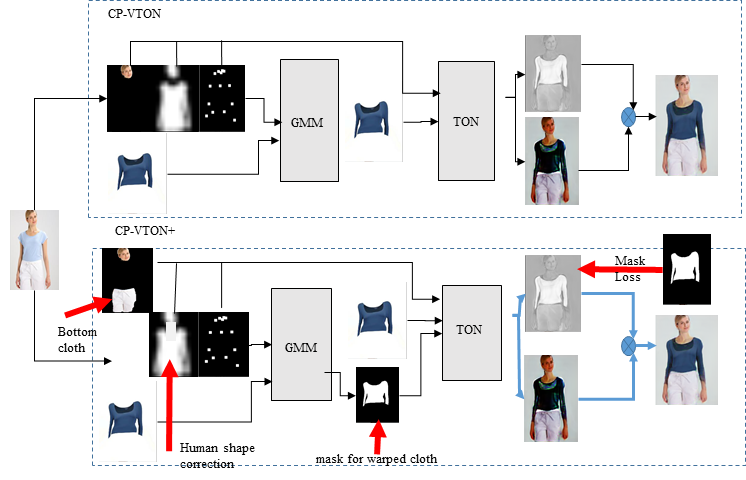
\includegraphics[height=6.5cm, scale=1]{figures/cpvton+pipeline.png}   
\caption{Full pipeline Comparison: CP-VTON and CP-VTON+: TODO: UPDATE with some more detailed one!!!}
\label{fig:piepline}
\end{figure}

\subsubsection{Cloth Warping Stage}

The modification in GMM stage are three locations. 
% Correction on the cloth agnostic human representation:
First, It is crucial to obtain the complete target body area for the try-on cloth and the target area should be the current-cloth agnostic. As described above, the original VITON dataset does not satisfy this requirement. We define a segmentation correction process as follow.  
% BG2SKIN
To be independent upon the current cloth the human wear, a new label ‘skin’ is added to the label set, and then  the pixels wrongly labelled as 'background' in VITON dataset are replaced by 'skin' considering the joint locations. The skin-labelled area now is included in the silhouette in the human representation (Figure  ~\ref{fig:cpvtonissues} (a)).
% HAIR-OCCLUSION
To recover the hair occlusion over the body, first the hair occlusion area are identified as the intersection of convex contour of the upper cloth and the hair-labelled area, and the intersection are re-labelled as upper cloth.   
% @TODO!!
%\ref{fig:cpvtonissues} (a)).

% GIC Network modification: 
Second, CP-VTON GMM network is built on CNN geometric matching \cite{rocco2017convolutional}, and trained in self-supervised manner by the L1 loss between the warped cloth images and the current human cloth. It is quite interesting that CNN geometric matching uses a pair of color images, but CP-VTON GMM uses a human representation, e.g. silhouette and joint heatmap with the try-on cloth. The texture information from try-on cloth does not help in matching process, thus our GMM use $M_{C_i}$ instead of $C_i$, i.e.,  
\[  
   \bold{\theta} = f_{\theta} ( f_H (H_t), f_C(M_{C_i}) )
\]
%The human representation only provide the shape and structure information 
%and the try-on cloth provides both texture and shape information. 


Finally, the experiments above reveals the warped cloth often distorted severely. We tried to understand the origin of this distortion, but it is not easy to explain clearly.  However, we conclude that the TPS parameter estimation needs the regularization, taking into account the restriction of cloth textile. Our grid warping regularization is defined on the grid deformation not directly the TPS parameter for easy visualization and understanding,  not to have too much different warping from the before and next grid gap in equation ~\ref{eq:gridloss}.
\begin{equation}
 L_{GMM}^{CP-VTON+}  = \lambda_1 \cdot L1(C_{warped}, I_{C_t}) + lambda_2 \cdot  L_{reg}  
\end{equation}

%The comparison result \cite{fig:2dvton_same} and \cite{fig:2dvton_diff} shows the 


%, which again uses the spatial transform networks by Zimmerman et al.'s \cite{jaderberg2015spatial}. Although warping network can work in both instance-level and category-level, our experiments  reveals the warped cloth often distorted severely.


%Our finding is that the warping network try to matches cloth images with human representation of silhouette and joint heatmap. The latter does not have no texture features but the shape information. From the failure case examinations, we found that the warping in the failure case is often too extreme, so that we try to restrict the warping parameters. Instead of single step TPS warping, we designed 2 stage warping network, in the first stage it warped roughly with Affine transform, and in the second stage it warped delicately with TPS transform. Not to have un-realistic warping, we added warping regularization loss. In the second stage, the sizes of cloth and target area in the human representation are in the same scale, so that the matching network can find the matching better. 


\begin{equation}\label{eq:gridloss}
\begin{aligned}
 L_{reg} (G_x, G_y) = \sum_x \sum_y | G_x(x+1, y) - G_x(x, y) | - | G_x(x, y) - G_x(x-1, y) | \\
 + | G_y(x, y+1) - G_y(x, y) | - | G_y(x, y) - G_y(x, y-1) |
\end{aligned}
\end{equation}



\subsubsection{Blending Stage}

The modification to GMM stage are two locations.
%\begin{itemize}
%\item[$\bullet$] Retaining the remaining area except the target cloth  :
In order to retain the other human components except the target cloth area, e.g. bottom clothes and legs, the all other area except the target cloth area are added for the human representation input of TOM, along with face and hair (Figure ~\ref{fig:cpvtonissues} (c))

%\item[$\bullet$] Training Composition alpha-map:  
In the mask loss term in TOM loss function, we replaced the Composition Mask with supervised ground truth mask for a strong alpha mask.

\begin{equation}
 L_{TOM}^{CP-VTON+} = \lambda_{L1} || I_0-I_{GT}||_1+  \lambda_{VGG} L_{VGG} + \lambda_{mask} ||M_{GT}-M_o||_1       
\end{equation}

Also, we added the binary mask of warped cloth to TOM network input so that TOM can clearly differentiate the target cloth area regardless of cloth color.  

%\end{itemize}

%\begin{figure}
%\centering
%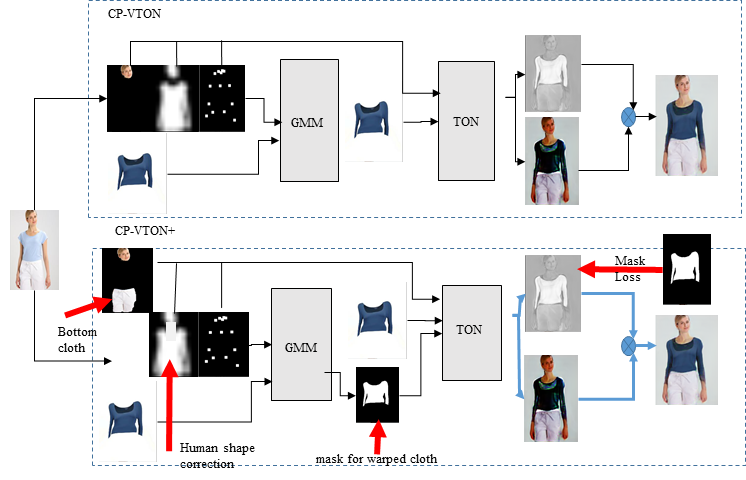
\includegraphics[height=6.5cm, scale=1]{figures/cpvton+pipeline.png}   
%\caption{2 stage GMM design with regularization loss}
%\label{fig:piepline}
%\end{figure}

